\subsection{Odzyskiwanie globalnych konturów z lokalnych cech}
\label{integracjaGPC}

W celu przeprowadzenia integracji konturów wcale nie trzeba budować sieci neuronowej tak jak to było pokazane w poprzednich częściach tej pracy. Autorzy pracy \cite{Guy1993} przedstawiają trochę inny punkt widzenia. Jako pierwsze wprowadzają pojęcie pola rozszerzenia\footnote{Z języka angielskiego -- extension field.} jako wzorca reprezentującego rodzinę gładkich krzywych.\\

Mimo, że w pracy autorzy nie skupiają się specjalnie na elementach, na których mają zamiar pracować -- twierdzą, że może to być poziom piksli jak i cech, czyli krawędzi w obrazie -- i raczej powinno się do tego podchodzić sceptycznie, to sama metoda może mieć sens, a obserwowane wyniki mogą napawać optymizmem.\\

Najprostszy opis metody polegałby na stwierdzeniu, że każdy element obrazu (piksel, bądź cecha -- zależnie od poziomu abstrakcji) jest określony poza swoimi zwykłymi parametrami pozwalającymi na zidentyfikowanie jego w obrazie (na przykład położenie) przez parametry takie jak kąt i siła. Są one ściśle przypisane do każdego segmentu -- na który cały obraz jest podzielony. Każdy segment zbiera informacje z innych segmentów, ze swojego otoczenia (zgodnie z konkretnymi wagami). Następnie liczona jest ,,zgodność wśród głosów'' z punktu widzenia orientacji segmentów. Spośród tych segmentów, te z wysoką oceną są nazywane istotnymi\footnote{Z języka angielskiego -- salient.}.\\

\subsubsection{Pole rozszerzenia}
\label{GPC_extensionField}

Przedstawione poniżej -- na rysunku \ref{fig:gpc_ef} -- pole rozszerzenia przedstawia zakres wpływu sąsiednich elementów krawędziowych na jeden konkretny. Co autorzy cytowanej pracy podkreślali istotny jest jedynie pozytywny wpływ, czyli nie ma możliwości wpływania negatywnego na wynik -- siłę, jaka zostanie danemu elementowi krawędziowemu przypisana. Czego wprawdzie nie widać na załączonym rysunku, to fakt, że teoretycznie zakres wpływu na element krawędziowy jest nieograniczony. \\

\begin{figure}[ht]
	\centering
	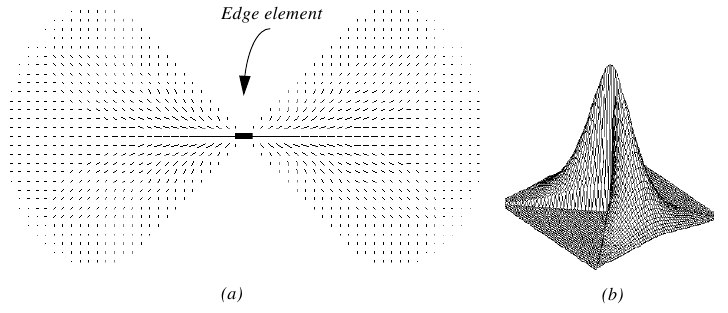
\includegraphics[width=1\textwidth]{images/gpc_ef.png}
	\caption{Pole rozszerzenia opisujące wpływ sąsiednich segmentów na jeden konkretny ze względu na (a) kąt oraz (b) siłę \cite{Guy1993}.}
	\label{fig:gpc_ef}
\end{figure}

Należy również przedstawić sytuacje, w których segmenty krawędziowe będą w pewnej istotnej\footnote{Takiej, że będzie ona miała znaczący wpływ na brany pod uwagę inny element krawędziowy.} odległości od siebie. Złączenie pól rozszerzenia pokaże wtedy jak jest interpretowany związek tych dwóch elementów krawędziowych i to w jaki sposób będzie uogólniana część krzywej, która mogłaby je łączyć. Rysunek \ref{fig:gpc_2ef} przedstawia taką właśnie sytuację.

\begin{figure}[ht]
	\centering
	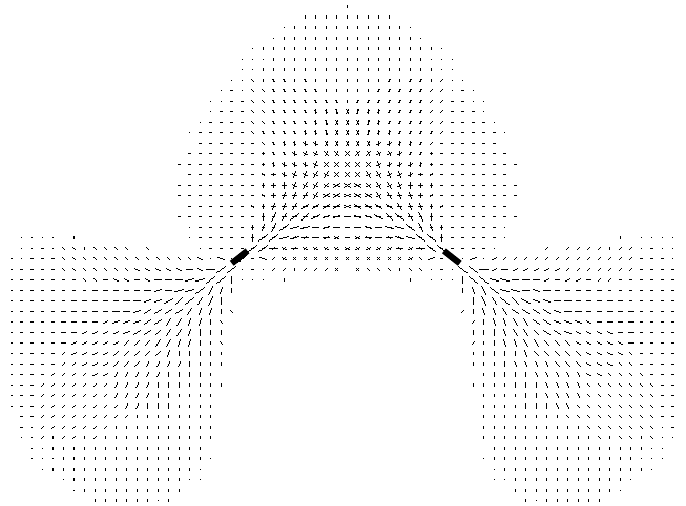
\includegraphics[width=.9\textwidth]{images/gpc_2ef.png}
	\caption{Wzajemny wpływ dwóch pól rozszerzenia na siebie i krzywa która jest na tej podstawie wydobywana \cite{Guy1993}.}
	\label{fig:gpc_2ef}
\end{figure}

Przedstawiany model wprawdzie jest bardzo prosty -- mimo, że nie przytacza się w tej pracy całej teorii matematycznej, która za tym stoi -- ale wyniki, jakie można osiągnąć przetwarzając obrazy przedstawione w różnej formie są napawające optymizmem. Na rysunku \ref{fig:gpc_res_in} przedstawione są obrazy wejściowe (w formie krawędzi -- a i b, kropek -- c jak i obrazu -- d) natomiast na rysunku \ref{fig:gpc_res_out} widać otrzymywane rezultaty, będące przedstawione w postaci samej mapy istotności. 

\begin{figure}[ht]
	\centering
	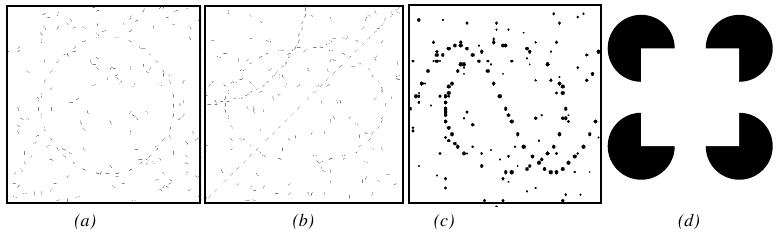
\includegraphics[width=.9\textwidth]{images/gpc_res_1.png}
	\caption{Obrazy wejściowe dla modelu \cite{Guy1993}.}
	\label{fig:gpc_res_in}
\end{figure}

\begin{figure}[ht]
	\centering
	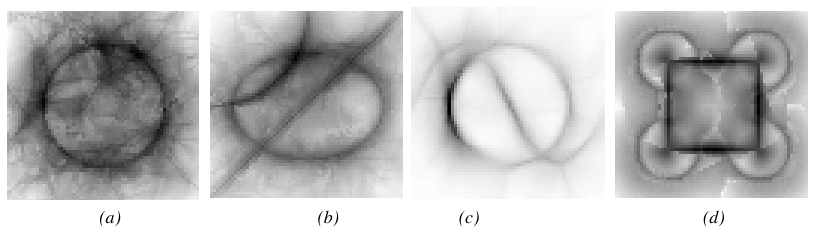
\includegraphics[width=.9\textwidth]{images/gpc_res_2.png}
	\caption{Otrzymywane wyniki przedstawione jako mapa istotności \cite{Guy1993}.}
	\label{fig:gpc_res_out}
\end{figure}

Po przetworzeniu tak przedstawionej mapy istotności do wyodrębnionych krawędzi można otrzymać obiecujące wyniki. Mimo, że w cytowanej pracy jest przedstawiony tylko jeden, to nic nie stoi na przeszkodzie, aby przypuszczać, że inne byłyby podobne. Ostateczny rezultat przedstawiony jest na rysunku \ref{fig:gpc_m_out}. Odpowiada on obrazowi wejściowemu \ref{fig:gpc_res_in}b oraz mapie istotności \ref{fig:gpc_res_out}b. Zdaniem autora niniejszej pracy bardziej efektowne byłoby przedstawienie obrazu \ref{fig:gpc_res_in}d po przetworzeniu przez model i pewnie zdanie czytelnika byłoby podobne, nie zmienia to jednak faktu, że w cytowanej pracy nie ma przedstawionych za pomocą krawędzi wyników modelu dla innych obrazów niż \ref{fig:gpc_res_in}b. Odnosi się bowiem wrażenie, że model jedynie pozbył się kilku nieistotnych zakłóceń w obrazie wejściowym.

\begin{figure}[ht]
  \centering
  \subfloat[Obraz wejściowy]{\label{fig:gpc_inn}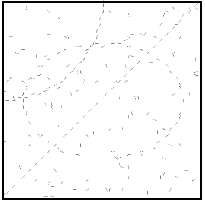
\includegraphics[width=0.3\textwidth]{images/gpc_res_model_in.png}}               
  \subfloat[Otrzymany wynik]{\label{fig:gpc_outt}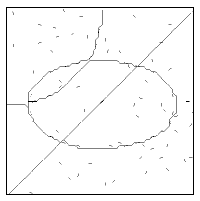
\includegraphics[width=0.3\textwidth]{images/gpc_res_model.png}}
  \caption{Wynik pracy modelu \ref{fig:gpc_outt} z obrazem \ref{fig:gpc_inn} przedstawiony w formie krawędzi. \cite{Guy1993}.}
  \label{fig:gpc_m_out}
\end{figure}


